% request-lifecycle.tex -- one GET through the middleware to the cache and back (ETag, 304), and the error path
% COS30049 Assignment 3, Bitcoin Address Activity Explorer. Drawn from the code on main (21 Nov 2026).
% Compiles on its own:  pdflatex request-lifecycle.tex   (one cropped page; needs only tikz and lmodern).
% It does not use the standalone class, which a small TeX installation may lack; the last lines of
% this file crop the page to the picture instead. To place it in the report: 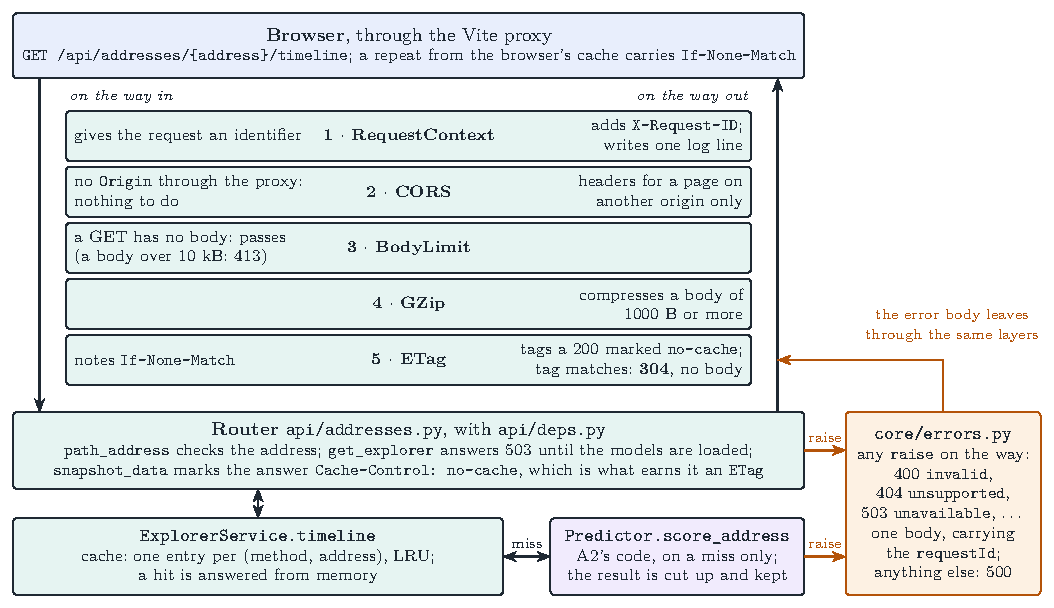
\includegraphics{request-lifecycle.pdf}.
% The boxes, words and arrows are the same as in request-lifecycle.svg; README.md lists the source file behind each.

\documentclass{article}
\usepackage[T1]{fontenc}
\usepackage{lmodern}
\usepackage{tikz}
\usetikzlibrary{arrows.meta, backgrounds}
% The plan's colours (docs/plan/main.tex).
\definecolor{ink}{HTML}{1F2933}
\definecolor{accent}{HTML}{1D4ED8}
\definecolor{accentsoft}{HTML}{E8EEFC}
\definecolor{teal}{HTML}{0F766E}
\definecolor{tealsoft}{HTML}{E6F4F2}
\definecolor{violet}{HTML}{6D28D9}
\definecolor{violetsoft}{HTML}{F1EBFD}
\definecolor{grey}{HTML}{6B7280}
\definecolor{greysoft}{HTML}{F3F4F6}
\definecolor{warn}{HTML}{B45309}
\definecolor{warnsoft}{HTML}{FDF1E3}
\pagestyle{empty}
\newsavebox{\figbox}
\newlength{\figborder}\setlength{\figborder}{6pt}
\begin{document}
\begin{lrbox}{\figbox}%
\frenchspacing
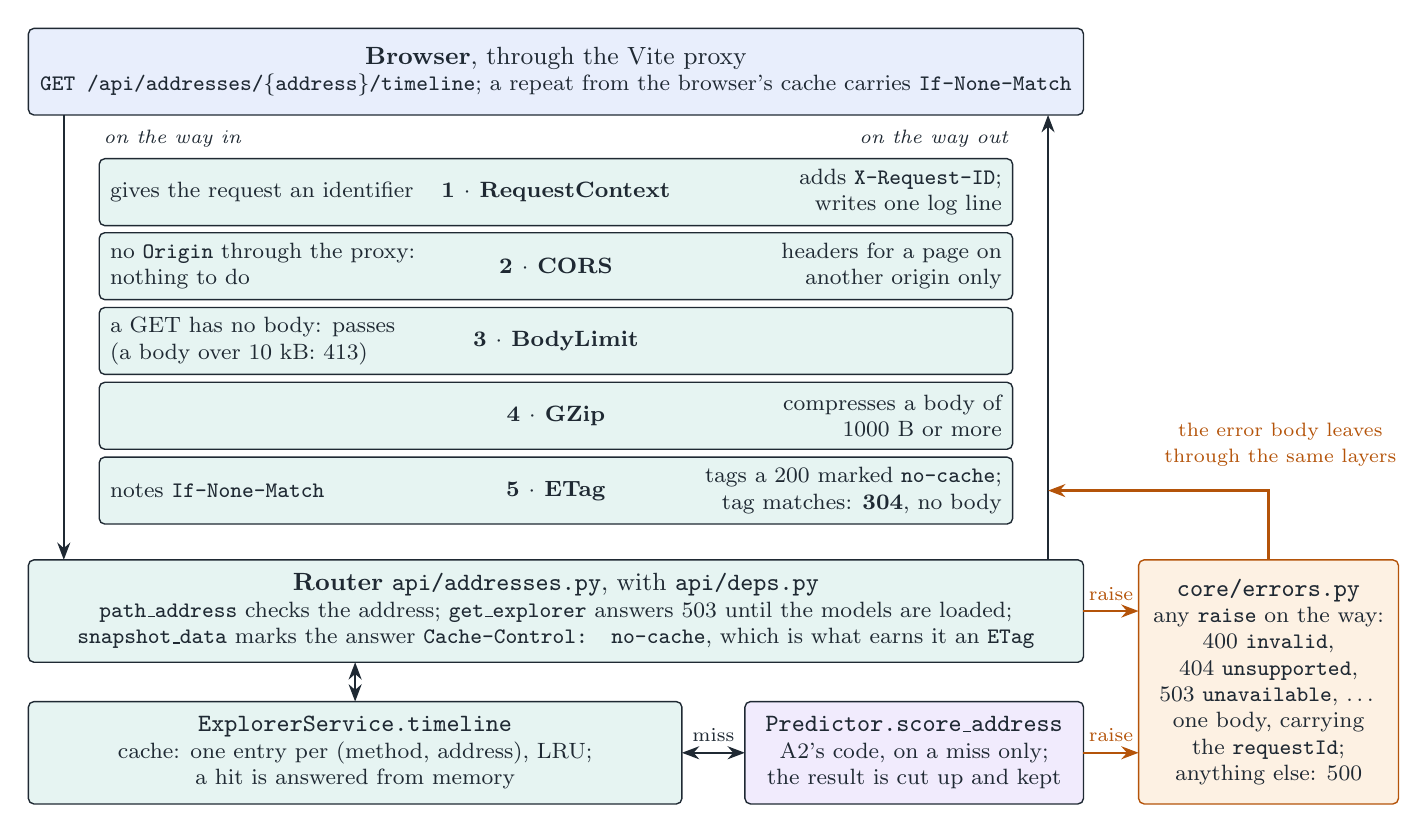
\begin{tikzpicture}[x=1cm, y=1cm, font=\footnotesize, text=ink,
  box/.style={draw=ink, rounded corners=2pt, align=center, inner sep=3pt, line width=0.5pt},
  fe/.style={box, fill=accentsoft}, be/.style={box, fill=tealsoft}, ml/.style={box, fill=violetsoft},
  st/.style={box, fill=greysoft}, er/.style={box, fill=warnsoft, draw=warn}, plain/.style={box, fill=white},
  txt/.style={align=center, inner sep=0pt},
  grp/.style={rounded corners=4pt, line width=0.6pt},
  arr/.style={-{Stealth[length=2.2mm]}, thick, draw=ink},
  darr/.style={{Stealth[length=2.2mm]}-{Stealth[length=2.2mm]}, thick, draw=ink},
  opt/.style={arr, dashed},
  err/.style={arr, draw=warn},
  bare/.style={thick, draw=ink}]
  % ---- groups (frames behind everything)
  % ---- boxes
  \node[fe, minimum width=13.40cm, minimum height=1.10cm] (browser) at (6.70,-0.55) {{\small \textbf{Browser}, through the Vite proxy}\\ \texttt{GET /api/addresses/\{address\}/timeline}; a repeat from the browser's cache carries \texttt{If-{}None-{}Match}};
  \node[be, minimum width=11.60cm, minimum height=0.85cm] (m1) at (6.70,-2.08) {\textbf{1 $\cdot$ RequestContext}};
  \node[txt, align=left, anchor=west] at (1.03,-2.08) {gives the request an identifier};
  \node[txt, align=right, anchor=east] at (12.37,-2.08) {adds \texttt{X-{}Request-{}ID};\\ writes one log line};
  \node[be, minimum width=11.60cm, minimum height=0.85cm] (m2) at (6.70,-3.02) {\textbf{2 $\cdot$ CORS}};
  \node[txt, align=left, anchor=west] at (1.03,-3.02) {no \texttt{Origin} through the proxy:\\ nothing to do};
  \node[txt, align=right, anchor=east] at (12.37,-3.02) {headers for a page on\\ another origin only};
  \node[be, minimum width=11.60cm, minimum height=0.85cm] (m3) at (6.70,-3.97) {\textbf{3 $\cdot$ BodyLimit}};
  \node[txt, align=left, anchor=west] at (1.03,-3.97) {a GET has no body: passes\\ (a body over 10 kB: 413)};
  \node[be, minimum width=11.60cm, minimum height=0.85cm] (m4) at (6.70,-4.92) {\textbf{4 $\cdot$ GZip}};
  \node[txt, align=right, anchor=east] at (12.37,-4.92) {compresses a body of\\ 1000 B or more};
  \node[be, minimum width=11.60cm, minimum height=0.85cm] (m5) at (6.70,-5.87) {\textbf{5 $\cdot$ ETag}};
  \node[txt, align=left, anchor=west] at (1.03,-5.87) {notes \texttt{If-{}None-{}Match}};
  \node[txt, align=right, anchor=east] at (12.37,-5.87) {tags a 200 marked \texttt{no-{}cache};\\ tag matches: \textbf{304}, no body};
  \node[be, minimum width=13.40cm, minimum height=1.30cm] (router) at (6.70,-7.40) {{\small \textbf{Router} \texttt{api/addresses.py}, with \texttt{api/deps.py}}\\ \texttt{path\_address} checks the address; \texttt{get\_explorer} answers 503 until the models are loaded;\\ \texttt{snapshot\_data} marks the answer \texttt{Cache-{}Control: no-{}cache}, which is what earns it an \texttt{ETag}};
  \node[be, minimum width=8.30cm, minimum height=1.30cm] (service) at (4.15,-9.20) {{\small \textbf{\texttt{ExplorerService.timeline}}}\\ cache: one entry per (method, address), LRU;\\ a hit is answered from memory};
  \node[ml, minimum width=4.30cm, minimum height=1.30cm] (a2) at (11.25,-9.20) {{\small \textbf{\texttt{Predictor.score\_address}}}\\ A2's code, on a miss only;\\ the result is cut up and kept};
  \node[er, minimum width=3.30cm, minimum height=3.10cm] (errors) at (15.75,-8.30) {{\small \textbf{\texttt{core/errors.py}}}\\ any \texttt{raise} on the way:\\ 400 \texttt{invalid},\\ 404 \texttt{unsupported},\\ 503 \texttt{unavailable}, \ldots{}\\ one body, carrying\\ the \texttt{requestId};\\ anything else: 500};
  % ---- arrows
  % request, inwards
  \draw[arr] (0.45,-1.10) -- (0.45,-6.75);
  % response, outwards
  \draw[arr] (12.95,-6.75) -- (12.95,-1.10);
  % router <-> service
  \draw[darr] (4.15,-8.05) -- (4.15,-8.55);
  % service <-> A2 on a miss
  \draw[darr] (8.30,-9.20) -- (9.10,-9.20);
  % router/deps raise
  \draw[err] (13.40,-7.40) -- (14.10,-7.40);
  % service / A2 raise
  \draw[err] (13.40,-9.20) -- (14.10,-9.20);
  % error body joins the way out
  \draw[err] (15.75,-6.75) -- (15.75,-5.87) -- (12.95,-5.87);
  % ---- labels
  \node[txt, anchor=west, font=\scriptsize] at (0.95,-1.40) {\itshape on the way in};
  \node[txt, anchor=east, font=\scriptsize] at (12.45,-1.40) {\itshape on the way out};
  \node[txt, font=\scriptsize] at (8.70,-8.98) {miss};
  \node[txt, text=warn, font=\scriptsize] at (13.75,-7.18) {raise};
  \node[txt, text=warn, font=\scriptsize] at (13.75,-8.98) {raise};
  \node[txt, text=warn, font=\scriptsize] at (15.90,-5.12) {the error body leaves};
  \node[txt, text=warn, font=\scriptsize] at (15.90,-5.45) {through the same layers};
\end{tikzpicture}%
\end{lrbox}
% One page, cropped to the picture plus a 6 pt border (what the standalone class would do).
\pdfpagewidth=\dimexpr\wd\figbox+2\figborder\relax
\pdfpageheight=\dimexpr\ht\figbox+\dp\figbox+2\figborder\relax
\pdfhorigin=\figborder \pdfvorigin=\figborder
\hoffset=0pt \voffset=0pt
\shipout\vbox{\box\figbox}
\end{document}
